\documentclass[12pt]{article}

\usepackage[T2A]{fontenc}
\usepackage[utf8]{inputenc}
\usepackage[english, russian]{babel}

\usepackage[letterpaper,top=2cm,bottom=2cm,left=1.5cm,right=1.5cm,marginparwidth=1.75cm]{geometry}
\usepackage{float}
%\usepackage[stable]{footmisc}

\usepackage{amsmath,amssymb}
\usepackage{graphicx}
\usepackage[colorlinks=true, allcolors=blue]{hyperref}
\hypersetup{unicode=true}
\usepackage{url}
\usepackage{longtable,booktabs,array}
\usepackage{tablefootnote}
\usepackage{circuitikz}
\usetikzlibrary{fit}

\title{Лабораторная работа № 3 \\
``Оптические датчики измерения расстояния. Инфракрасный дальномер'' \\
\large Сенсоры и сенсорные системы}

\begin{document}
\maketitle
\tableofcontents
\begin{abstract}
    Оптический инфракрасный дальномер. Принцип работы. Определение функциональной зависимости расстояния от выходного сигнала датчика.
\end{abstract}

\section{Теория}

Оптические методы измерения расстояния до объектов построены на анализе отраженного светового сигнала от объекта. Инфракрасные (infra-red, IR) дальномеры (рис.~\ref{sharp}) работают по принципу триангуляции, то есть измерения угла падения отраженного света от объекта. Угол падения зависит от расстояния от излучателя до объекта. Датчик излучает узкий световой луч IR-светодиодом через лизну, которая называется \textit{Light emitter} (см. рис.~\ref{light}). Отраженный от объекта световой сигнал поступает на приемную собирающую линзу (\textit{Light detector}). После сфокусированный световой луч попадает на позиционно-чувствительное устройство PSD (\textit{Position Sensitive Device}), образуя световое пятно на плоскости чувствительности PSD, которое меняет свое положение в зависимости от угла падения. От местоположения светового пятна на чувствительной плоскости PSD в свою очередь зависит его проводимость, в следствии чего изменяется выходное напряжение датчика. Соответственно, расстояние от излучателя до объекта зависит от выходного напряжения датчика, т.е., расстояние \(S\) есть функция от выходного напряжения \(V_{o}\):
\[S=f(V_{o}).\]

\begin{figure}[H]
    \centering
    \begin{minipage}[H]{0.49\linewidth}
        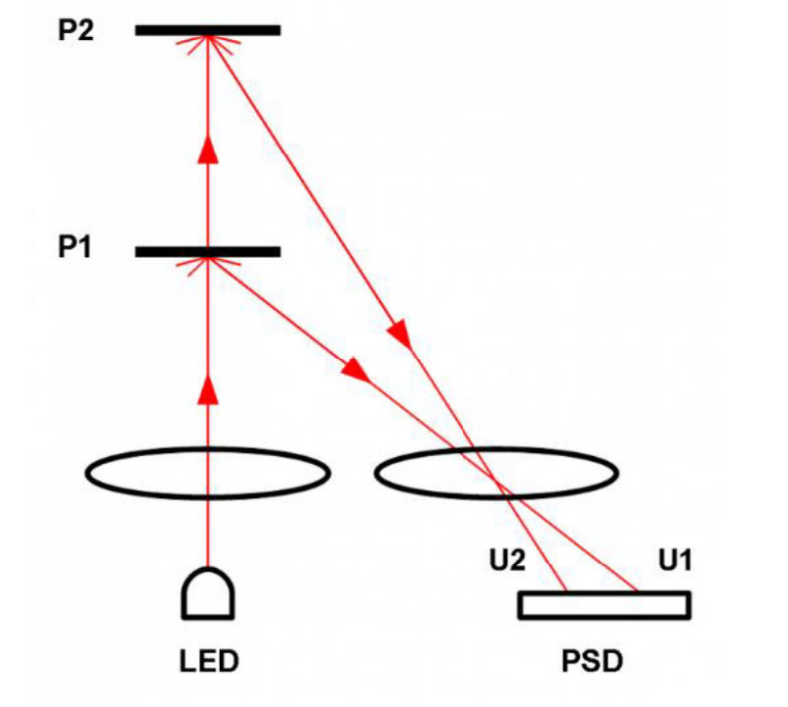
\includegraphics[scale=0.5]{images/light.png}
        \caption{Путь светового луча инфракрасного \\ дальномера}\label{light}
    \end{minipage}
    \begin{minipage}[H]{0.49\linewidth}
        \begin{tikzpicture}[>=latex]
            \draw (0, 0) node[inner sep=0]{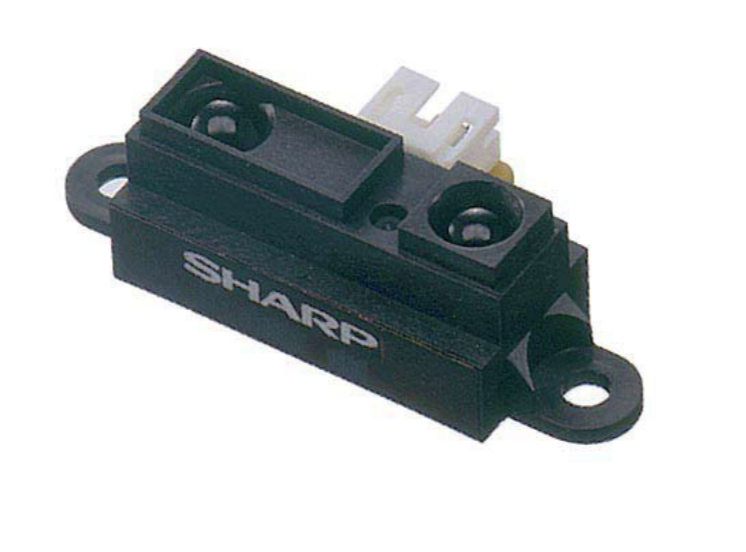
\includegraphics[scale=0.55]{images/GP2Y0A21YK0F.png}};
            \draw[thick, ->, red] (3, 3) node[above]{Light emitter} -- (1.3,0.5);
            \draw[thick, ->, red] (-3, 3.5) node[above]{Light detector} -- (-2, 2);
        \end{tikzpicture}
        \caption{Внешний вид IR-дальномера производства компании Sharp}\label{sharp}
    \end{minipage}
\end{figure}

\subsection[Подробнее о позиционно-чувствительном устройстве PSD]{Подробнее о позиционно-чувствительном устройстве PSD\footnote{Источник: \url{https://www.wikiwand.com/en/Position_sensitive_device}}}


\textbf{Позиционно-чувствительное устройство} (англ. Position Sensitive Device, PSD) \textbf{позиционно-чувствительный детектор} (англ. Position Sensitive Detector, PSD) — оптический датчик, способный измерять положение светового пятна на поверхности датчика в одном или двух измерениях.

В соответствии со структурой позиционно-чувствительные устройства разделяют на два вида:
\begin{itemize}
    \item устройства с однородной поверхностью датчика. Производят непрерывные (аналоговые) данные о положении.
    \item устройства на базе множества дискретных сенсоров, упорядоченно расположенных на поверхности датчика. Производят дискретные (цифровые) данные о положении.
\end{itemize}

\textbf{Аналоговые PSD}

Технический термин PSD впервые был использован в публикации 1957 года Дж.Т. Уоллмарком для бокового фотоэлектрического эффекта, используемого для локальных измерений. Ламинарный полупроводник (рис.~\ref{psd}), так называемый контактный диод, подвергается воздействию крошечного светового пятна. Это воздействие вызывает изменение местного сопротивления и, следовательно, потока электронов в четырех электродах. 

\begin{figure}[H]
    \centering
    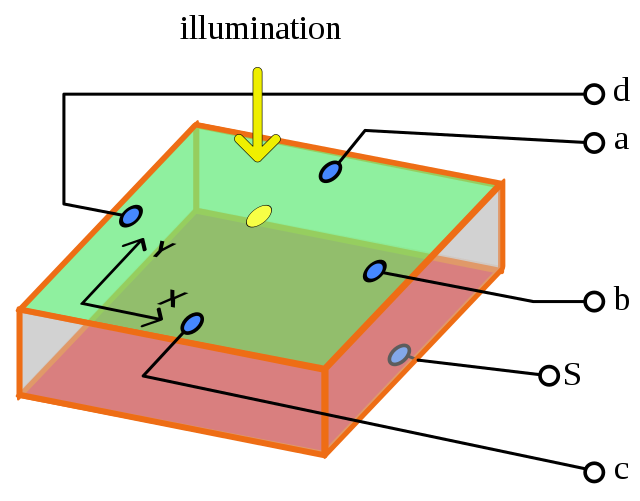
\includegraphics[scale=0.4]{images/psd.png}
    \caption{Аналоговой позиционно-чувствительный детектор}\label{psd}
\end{figure}

Исходя из токов \(I_{a}\), \(I_{b}\), \(I_{c}\) и \(I_{d}\) в электродах, местоположение светового пятна вычисляется с использованием следующих уравнений:
\[x=k_{x}\cdot\frac{I_{b}-I_{d}}{I_{b}+I_{d}},\]
и
\[x=k_{x}\cdot\frac{I_{a}-I_{c}}{I_{a}+I_{c}},\]
где \(k_{x}\) и \(k_{y}\) - коэффициенты масштабирования по осям.

Преимуществом аналоговых PSD заключается в непрерывном измерение положения светового пятна со частотой до 100 кГц. Зависимость локального измерения от формы и размера светового пятна, а также нелинейного соединения является недостатком, который может быть частично компенсирован специальными формами электродов.

\textbf{Дискретные PSD}

\textit{Последовательная обработка}. Наиболее распространенные сенсорные приложения с частотой дискретизации менее 1000 Гц - это CCD или CMOS камеры. Датчик разделен на отдельные пиксели, значение экспозиции которых можно считывать последовательно. Положение светового пятна можно рассчитать методами фотограмметрии непосредственно по распределению яркости.

\textit{Параллельная обработка} (рис.~\ref{psddiscrete}). Для более быстрых применений были разработаны матричные датчики с параллельной обработкой. И построчно, и в столбцах плотность света каждого пикселя сравнивается с глобальным пороговым значением. Результатами сравнения становятся строки и столбцы с логическими элементами ИЛИ. Из всех столбцов и всех строк один элемент, который ярче заданного порогового значения, представляет собой среднее значение координат, вычисленных для светового пятна.

\begin{figure}[H]
    \centering
    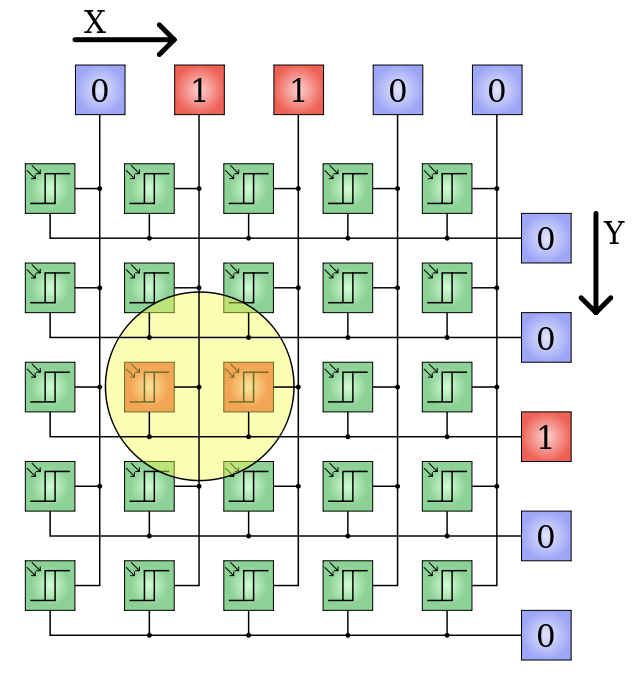
\includegraphics[scale=0.3]{images/psd-discrete.png}
    \caption{Дискретный PSD с параллельной обработкой}\label{psddiscrete}
\end{figure}

\subsection{IR-дальномер GP2Y0A21YK0F}
В данной работе рассматривается IR-дальномер GP2Y0A21YK0F производства комании Sharp. Его характеристики представлены ниже в таблице~\ref{techspec}.

\begin{table}[H]
    \centering
    \caption{Характеристики GP2Y0A21YK0F}\label{techspec}
    \begin{tabular}{c|c}
        \toprule
        Диапазон измерений расстояния, см & 8-10 \\
        \hline
        Типа выхода & Аналоговый 0,4 В (80 см) - 2,3 В (10 см) \\
        \hline
        Напряжение питания, В & 4,5-5,5 \\
        \hline
        Ток потребления, мА & 30 мА \\
        \bottomrule
    \end{tabular}
\end{table}

Блок схема внутренней структуры датчика GP2Y0A21YK0F приведена на рис.~\ref{blockscheme}. 

\begin{figure}[H]
    \centering
    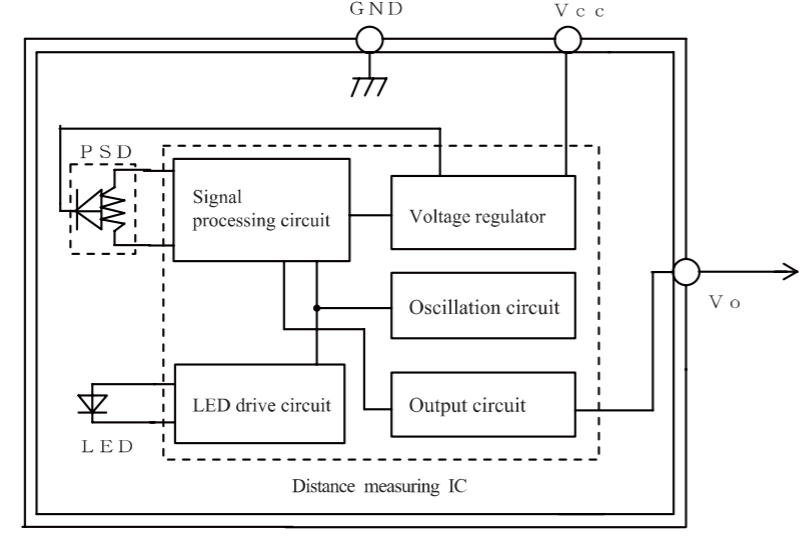
\includegraphics[scale=0.6]{images/block-scheme.png}
    \caption{Структура IR-двльномера GP2Y0A21YK0F}\label{blockscheme}
\end{figure}

Выходное напряжение датчика обратно зависит от измеряемого расстояния - с увеличением расстояния выходное напряжение снижается. График зависимости выходного напряжения \(V_o\) от расстояния \(S\) представлен на рис.~\ref{vlplot} (a). Функциональная связь \(V_o=f^{-1}(S)\) между напряжением и расстоянием нелинейная, что видно по кривизне графика. 

У датчиков имеется граница измерения, в пределах которой выход датчика является достоверным. Измерение максимального расстояния ограничивается двумя факторами: уменьшение интенсивности отражающегося света и невозможность PSD регистрировать изменение местоположения отображенного светового луча (выход за границы чувствительного элемента). При измерении сильно удаленных объектов (дальше предела измерения), выходное напряжение датчика почти не изменяется. Минимально измеряемое расстояние ограничено зоной нечувствительности (резкий спад слева на графике (а)), то есть, при расстоянии до объекта меньше чем нижний предел измерения выходное напряжение прекратит закономерно возрастать и начнет резко падать при дальнейшем уменьшении расстояния. Поэтому измерений дальности датчиком будет адекватным только в пределах его диапазона.

\begin{figure}[H]
    \centering
    \begin{minipage}[H]{0.49\linewidth}
        \center{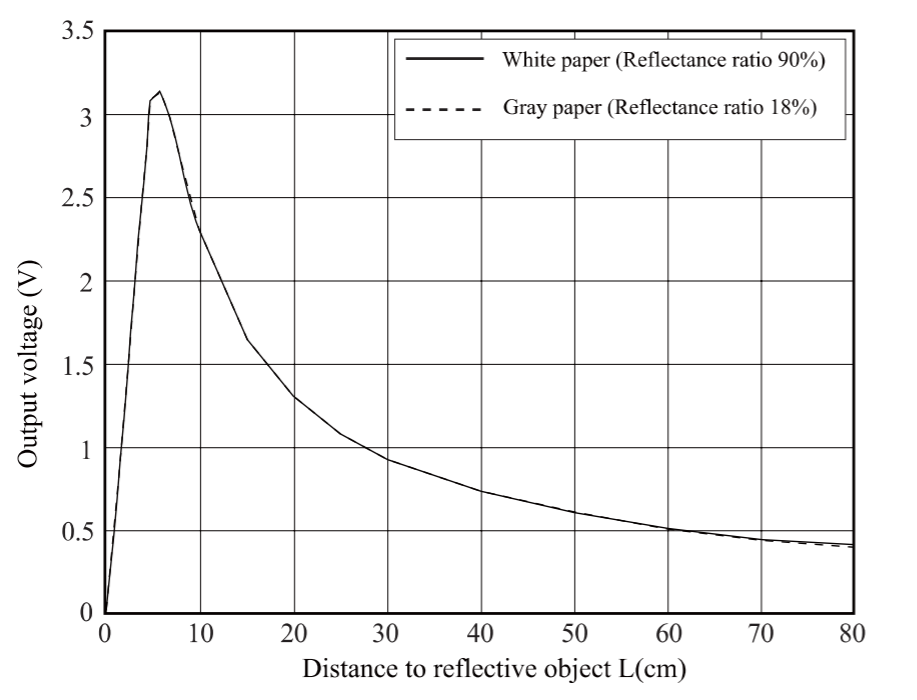
\includegraphics[scale=0.45]{images/VL-plot.png} \\ a)}
    \end{minipage}
    \begin{minipage}[H]{0.49\linewidth}
        \center{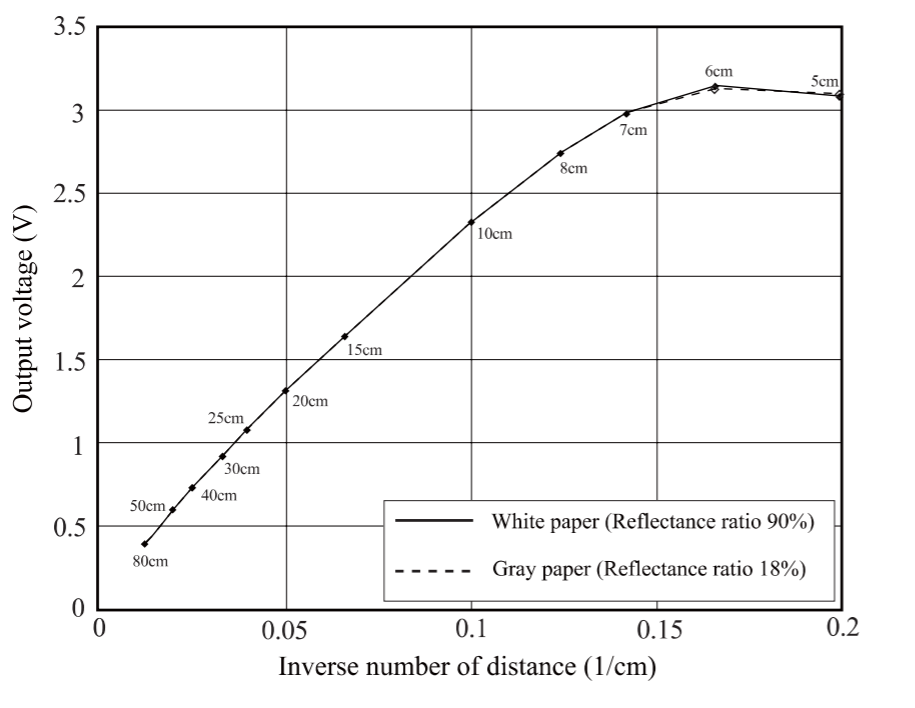
\includegraphics[scale=0.45]{images/VinvL-plot.png} \\ б)}
    \end{minipage}
    \caption{Характеристика датчика GP2Y0A21YK0F: a) зависимость выходного напряжения от расстояния \(S\), б) от обратного расстояния \(1/S\)}\label{vlplot}
\end{figure}

\subsection{Аппроксимация характеристики IR-дальномера}

На рис.~\ref{vlplot} (б) представлен график зависимости выходного напряжения \(V_o\) от обратного расстояния \(1/S\):
\[V_o=g\left(\frac{1}{S}\right).\]
В таком виде характеристика датчика принимает линейный вид в пределах диапазона измерения 10-80 см. По горизонтальной оси откладываются значения обратных расстояний от \(1/80=0,0125\) до \(1/10=0,1\), а по вертикальной оси соотвествующее им выходное напряжения датчика \(V_o\).

На практике чаще используют именно характеристику датчика от обратного расстояния, так как она близка к линейное в рабочем диапазоне датчика, что позволяет применить простую линейную аппроксимацию функциональной зависимости \(V_o=g\left(1/S\right).\) (приблизительная оценка функции \(g(\cdot)\)), чтобы использовать её в программном обеспечении для вычисления расстояния.

Процесс аппроксимации характеристики \(V_o=g\left(1/S\right).\) начинается с проведения эксперимента, когда измеряют выходное напряжения \(V_o\) с датчика при различном расстоянии \(S\) в пределах допустимого диапазона измерения. В результате получаются пар измерений \((V_o, S)\). Затем получают другой набор пар измерений с обратными напряжениями \((V_o, S^*)\), где  \(S^*=1/S\). Аппроксимирующую функцию ищут в виде линейной функции:
\begin{equation}
    V_o=g(S^*)=k\cdot S^*+b,
    \label{eq:eq1}
\end{equation}
где \(k\) и \(b\) подлежат оценки. 

После из найденной аппроксимирующей функции \(V_o=g(S^*)\) выражается \(S^*\), т.е.:
\[
    S^*=g^{-1}(V_o)=\frac{V_o-b}{k}.
\]
Учитывая \(S^*=1/S\), получим непосредственно искомую функцию зависимости расстояния до объекта от выходного напряжения:
\begin{equation}
    S=\frac{k}{V_o-b}.
    \label{eq:eq0}
\end{equation}

Оценка параметров \(k\) и \(b\) линейной функции происходит по измерениям выходного напряжения \(V_o\) при различнх расстояниях \(S\). В результате \(N\) измерений получаем \(N\) точек-пар \((V_o(i),\: S^*(i))\), \(i=\overline{1,\:N}\), \(S^*(i)=1/S(i)\). Для каждой \(i\)-ой пары измерений можно записать уравнение~(\ref{eq:eq1}):
\[
    V_o(i)=k\cdot S^*(i)+b.
\]

Уравнения для всех точек \(N\) образует систему \(N\) уравнения относительно двух неизвестных параметров \(k\) и \(b\), т.е.:
\[
    \begin{cases}
        V_o(1)=k\cdot S^*(1)+b \\
        V_o(2)=k\cdot S^*(2)+b \\
        V_o(3)=k\cdot S^*(3)+b \\
        \cdots \\
        V_o(N)=k\cdot S^*(N)+b.
    \end{cases}.
\]
Эту систему можно записать в векторно-матричном виде
\begin{equation}
    A\cdot 
    \begin{bmatrix}
        k \\ b
    \end{bmatrix}
    =P,
    \label{eq:eq2}
\end{equation}
где
\[
    A=
    \begin{bmatrix}
        S^*(1) & 1 \\
        S^*(2) & 1 \\
        S^*(3) & 1 \\
        \cdots \\
        S^*(N) & 1
    \end{bmatrix},
    \qquad
    P=
    \begin{bmatrix}
        V_o(1) \\
        V_o(2) \\
        V_o(3) \\
        \cdots \\
        V_o(N)
    \end{bmatrix} - 
\]
матрицы, получаемые из \(N\) измерений \((V_o(i),\: S^*(i))\).

Матричное уравние~(\ref{eq:eq2}) относительно вектора искомых параметров \(k\) и \(b\) решается следующим образом:
\begin{equation}
    \begin{bmatrix}
        k \\ b
    \end{bmatrix}
    =\left(A^T A\right)^{-1}A^T \cdot P.
    \label{eq:eq3}
\end{equation}
Найденные параметры \(k\) и \(b\) (1-ый и 2-ой элементы расчитанного вектора) можно использовать в искомой зависимости~(\ref{eq:eq0}) расстояния \(S\) от выходного напряжения \(V_o\).

\section{Лабораторная работа}
\subsection{Цель работы}
Изучить принцип действия оптического IR-дальномера. Проанализировать его характеристику. Провести экпериментальные измерения и аппроксимировать полученную характеристику датчика для получения аналитической формулы вычисления расстояния от выходного напряжения датчика.

\subsection{Оборудование}
Модуль датчиков. Модуль ``Микроконтроллер ATMEGA32'', компьютер/ноутбук. Рулетка или линейка не менее 80 см. Плоский предмет.

\subsection{Ход работы}
\subsubsection{Подключение}
Подключите модуль ``Микроконтроллер ATMEGA32'', модуль ``Модуль датчиков'' к внешнему блоку питания (или у портам USB компьютера/ноутбука) с помощью кабеля USB. Выполните коммутацию модулей приборными проводами в соответствии с таблицей~\ref{labtable}  и с рис.~\ref{labscheme}.

\begin{figure}[H]
    \centering
    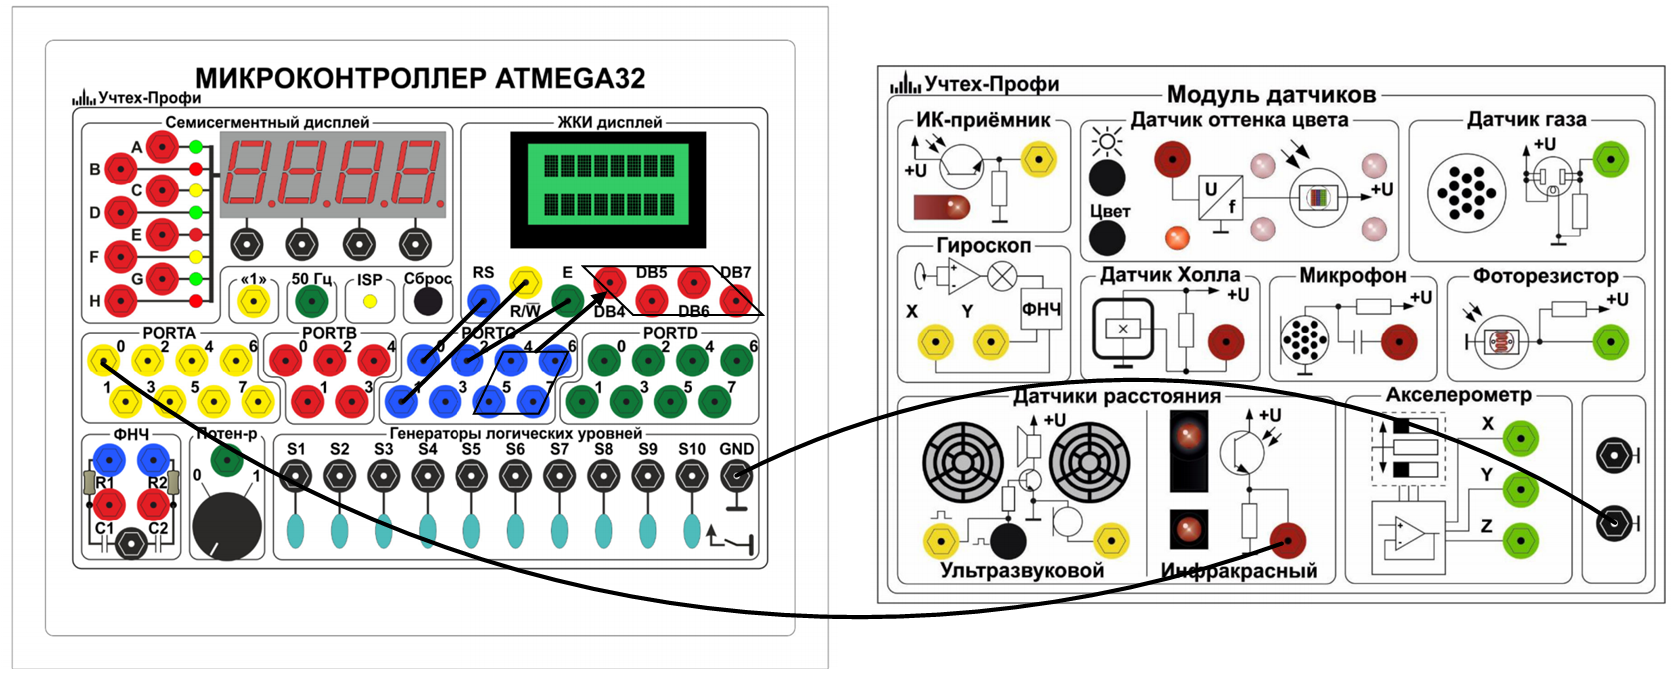
\includegraphics[scale=0.65]{images/lab3-scheme.png}
    \caption{Схема подключения модулей}\label{labscheme}
\end{figure}
\begin{table}[H]
    \caption{Коммутация модулей}\label{labtable}
    \begin{longtable}[]{@{}l|l@{}}
        \toprule
        Порт микроконтроллера ATMEGA32 & Назначение \\
        \midrule
        \endhead
        PORTC:0 & ЖК-дисплей: RS \\
        PORTC:1 & ЖК-дисплей: R/W \\
        PORTC:2 & ЖК-дисплей: E \\
        PORTC:4-7 & ЖК-дисплей: DB4-DB7 \\
        PORTA:0 & Инфракрасный дальномер \\
        \bottomrule
    \end{longtable}  
\end{table}

\subsubsection{Использование кода}

Для проведения измерений в лабораторной работе необходимо загрузить программу в микроконтроллер ATMEGA32. В папке \texttt{/src} лежат файлы исходного кода программы. Заголовочные файлы подключаемых модулей находятся \texttt{/include}. Основной выполняемый код находится в файле \texttt{/src/main.cpp}. Откройте его и проанализируйте код, который в нём содержится.

Запустите компиляцию и сборку прошивки нажав на кнопку ``Build'' на нижней панели VSCode. Затем загрузите файл прошивки в память микроконтроллера нажав на кнопку ``Upload''. После этого на ЖК-дисплее отобразятся измеряемое выходное напряжение \(V_o\) в мВ с IR-дальномера, которое зависит от расстояния \(S\) до плоского предмета.

\subsubsection{Проведение измерений}
Необходимо получить \(N=10\) измерений выходного напряжения \(V_o\) при различном расстоянии от датчика до плоского предмета в предалах рабочего диапазона 10-80 см. Испольуйте рулекту для измерения расстояния.

Заполните таблицу~\ref{exper}, где каждому расстоянию \(S(i)\) и обратному расстоянию \(S^*(i)=1/S(i)\) соответствует выходное напряжение датчика \(V_o(i)\), \(i=\overline{1,\:10}\) 

\begin{table}[H]
    \centering
    \caption{Экспериментальные измерения \(S\) и \(V_o\)}\label{exper}
    \begin{longtable}{c|c|c|c}
        \toprule
        № измерения \(i\) & \(S\), см & \(S^*=1/S\), 1/см & \(V_o\), мВ \\
        \midrule
        1 &&& \\
        \hline
        2 &&& \\
        \hline
        3 &&& \\
        \hline
        \dots &&& \\
        \hline
        10 &&& \\
        \bottomrule
    \end{longtable}
\end{table}

\subsubsection{Обработка измерений}

\begin{enumerate}
    \item Постройте графики экспериментально полученных зависимостей \(V_o=f(S)\) и \(V_o=g(1/S)\). Графики должны быть схожи с теми, которые представлены на рис.~\ref{vlplot}.
    \item Аппроксимация измерений. Для оценки параметров \(k\) и \(b\) искомой зависимости~(\ref{eq:eq0}) по экспериментальным измерениям (таблица~\ref{exper}) сформируйте матрицы \(A\) и \(P\) как показано в~(\ref{eq:eq2}). В результате должны быть получены матрицы размерностей 10х2 и 10х1 соответственно из измерений \(V_o(i)\) и \(S^*(i)\). Затем найдите вектор параметров \(k\) и \(b\) по формуле~\ref{eq:eq3}, воспользовавшись каким-нибудь мат-пакетом (например MatLab, MathCad).
    \item Запишите окончательный вид функциональной зависимости, подставим найденные параметры \(k\) и \(b\) в формулу~(\ref{eq:eq0}). График этой функции изобразите вместе с графиком из п. 1.
\end{enumerate}

\subsection{Вопросы}

\begin{enumerate}
    \item Принцип работы оптического IR-дальномера. Что такое и как работает позиционно-\\чувствительный детектор PSD?
    \item Вид характеристики IR-дальномера. Почему используется характеристика от обратного расстояния \(1/S\)?
    \item Алгоритм аппроксимации экспериментально полученной характеристики дальномера.
\end{enumerate}


\end{document}